\begin{figure}[t]
  % \vspace{-2em}
  \centering
  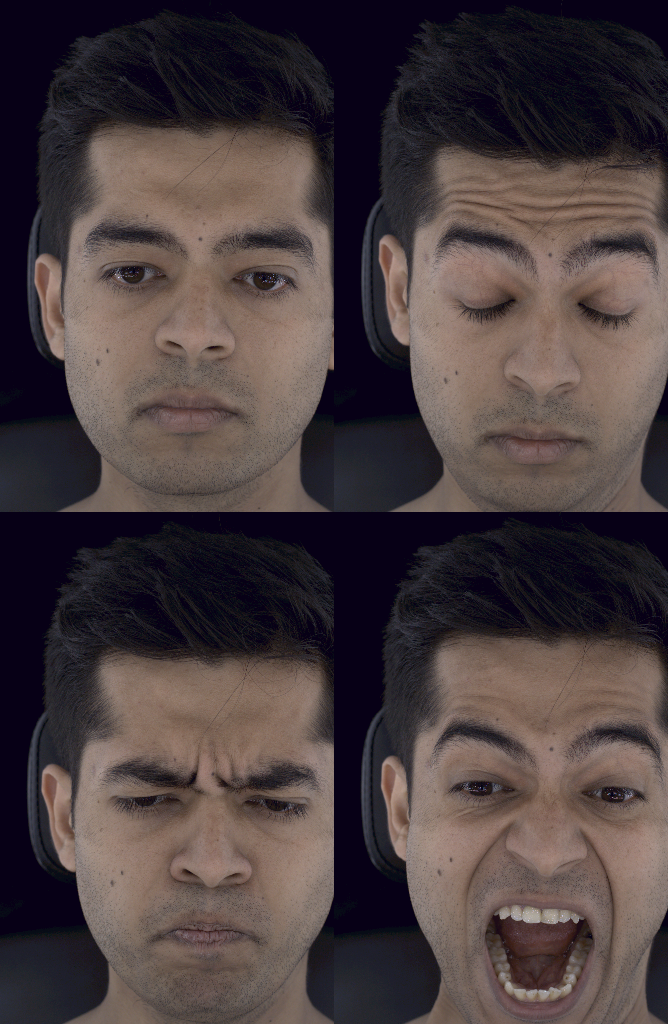
\includegraphics[width=0.7\linewidth,trim={0 2em 0 2em}, clip]{assets/\blendfieldsdirname/rebuttal/frames.png}
  \caption{\textbf{Training frames} -- In~\cref{sec:blendfields-experiments}, we show results for the \blendfields trained on $\nExpr{=}5$ expressions.
    The images represent these expressions for one of the subjects.
    For each subject, we selected similar expressions to show all possible
    wrinkles when combined.
    Please note that we also include a ``neutral'' expression (the first from
    the left)---it is necessary to enable the learning of a face without any
    wrinkles.
    % model to learn 
  }
  \label{fig:blendfields-supplementary-training-frames}
\end{figure}